\section{Fragments}

The player has the possibility to see stats for players, monsters and items.
He can also see all the items each player has gathered. An example of how the fragment is shown to the user is on figure \ref{fig:fragmentOverview} and \ref{fig:fragmentDetailed}.


\begin{figure}[ht!]
	\centering
	\begin{minipage}[t]{0.48\textwidth}
		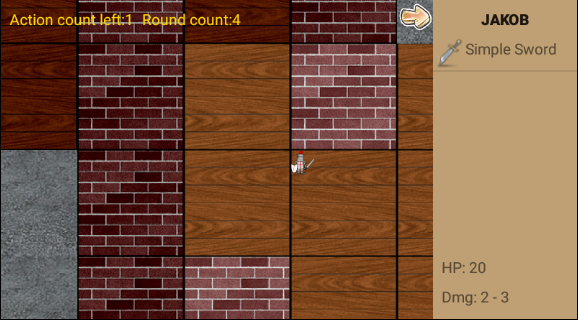
\includegraphics[width=\textwidth]{images/fragmentOverview.png}
		\caption{Overview fragment - Show the stats and items for a player}
		\label{fig:fragmentOverview}
	\end{minipage}
	\hfill
	\begin{minipage}[t]{0.48\textwidth}
		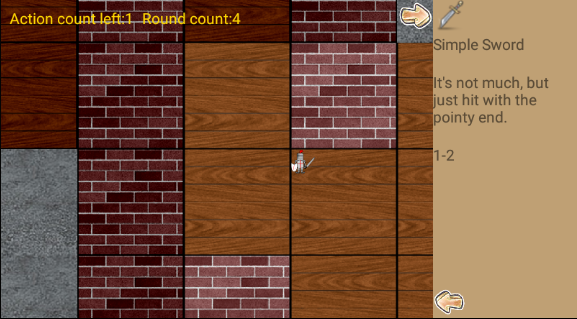
\includegraphics[width=\textwidth]{images/fragmentDetailed.png}
		\caption{Detailed fragment -  Shows stats for an specific item, when player click on an item in the overview fragment.}
		\label{fig:fragmentDetailed}
	\end{minipage}
\end{figure}

Depending on what the player want to see there are different ways to open the fragment view:\\
 - By clicking on the arrows in the top right corner (Shows the players own stats), or by clicking on the a monster or another player (Shows their stats). Both actions ends up calling a method in the GameView class. That method creates a new fragment and show it with an animation. \\
- If the fragment is showing the players item list, and the player clicks on an item it will when make a callback to the game activity. The game is then responsible for creating a new detailed fragment with the information, swapping it with the overview fragment. (See listing \ref{code:onItemSelected})

\begin{lstlisting}[language=Java, caption=onItemSelected method is called when a player clicks on an item in the overview fragment, label=code:onItemSelected]
public void onItemSelected(GameItem item) {
    Log.d("Item", "onItemSelected: Clicked!");
    overviewFragment = getSupportFragmentManager() .findFragmentById(R.id.game_board_activity_items_and_stats_fragment);
    detailFragment = fragment_item_details.newInstance((ItemWeapon) item);
    FragmentTransaction ft = getSupportFragmentManager().beginTransaction();
    ft.replace(R.id.game_board_activity_items_and_stats_fragment, detailFragment);
    ft.addToBackStack(null);
    ft.commit();
}
\end{lstlisting}